\begin{name}
{Đề Ôn Tập HS TB-Yếu}
{Năm học 2025-2026}
\end{name}

\Opensolutionfile{ans}[ans/De-TB-Yeu-So-17]
\cautn
\begin{ex} %[2H5N3-2]
	Trong không gian $Oxyz$, cho mặt cầu $(S)\colon \left(x-\sqrt{2}\right)^2+\left(y-\sqrt{5}\right)^2+\left(z+1\right)^2=\sqrt{10}$. Tâm của $(S)$ có tọa độ là
	\choice
	{$\left(-\sqrt{2};-\sqrt{5};1\right)$}
	{\True $\left(\sqrt{2};\sqrt{5};-1\right)$}
	{$\left(\sqrt{2};\sqrt{5};1\right)$}
	{$\left(-\sqrt{2};-\sqrt{5};-1\right)$}
	\loigiai{
		Tâm của mặt cầu $(S)$ có tọa độ là $\left(\sqrt{2};\sqrt{5};-1\right)$.
	}
\end{ex}

\begin{ex}%[2D1H3-1]
	Cho hàm số $y=f(x)$ có bảng biến thiên như hình vẽ.
	\begin{center}
		\begin{tikzpicture}
			\tkzTabInit[nocadre=false,lgt=1.2,espcl=3,deltacl=0.4]
			{$x$/0.75, $y'$/0.75, $y$/2.5}{$-\infty$,$-1$,$3$,$+\infty$}
			\tkzTabLine{,+,0,-,0,+,}
			\path
			(N13)node[shift={(0,0.4)}](A){$-4$}
			(N22)node[shift={(0,-0.4)}](B){$2$}
			(N33)node[shift={(0,0.4)}](C){$-3$}
			(N42)node[shift={(0,-0.6)}](D){$-1$}
			;
			\foreach\X/\Y in{A/B,B/C,C/D}\draw[-stealth](\X)--(\Y);
		\end{tikzpicture}
	\end{center}
	Giá trị nhỏ nhất của hàm số $f(x)$ trên đoạn $\left[0;4\right]$ là
	\choice
	{$f(0)$}
	{$-1$}
	{$-4$}
	{\True $-3$}
	\loigiai{
		Quan sát bảng biến thiên ta thấy giá trị nhỏ nhất của hàm số $f(x)$ trên đoạn $\left[0;4\right]$ là: $-3$.
	}
\end{ex}

\begin{ex}%[1D5H2-2]
	Giả sử nhóm $k$ là nhóm đầu tiên có tần số tích lũy lớn hơn hoặc bằng $\dfrac{n}{2}$, tức là $cf_{k-1}<\dfrac{n}{2}$ nhưng $cf_k\ge \dfrac{n}{2}$. Gọi $r$, $d$, $n_k$ lần lượt là đầu mút trái, độ dài, tần số của nhóm $k$; $cf_{k-1}$ là tần số tích lũy của nhóm $k-1$. Công thức trung vị nào sau đây là đúng?
	\choice
	{$M_e=d+\left(\dfrac{\dfrac{n}{2}-cf_{k-1}}{n_k}\right)\cdot r$}
	{\True $M_e=r+\left(\dfrac{\dfrac{n}{2}-cf_{k-1}}{n_k}\right)\cdot d$}
	{$M_e=r+\left(\dfrac{\dfrac{n}{2}+cf_{k-1}}{n_k}\right)\cdot d$}
	{$M_e=d+\left(\dfrac{\dfrac{n}{2}+cf_{k-1}}{n_k}\right)\cdot r$}
	\loigiai{
	Ta có $M_e=r+\left(\dfrac{\dfrac{n}{2}-cf_{k-1}}{n_k}\right)\cdot d$.
	}
\end{ex}

\begin{ex}%[2D4H3-1]
	Diện tích hình phẳng giới hạn bởi hai parabol $y=x^2+3x-1$ và $y=-x^2+x+3$ được tô đậm trong hình bên có giá trị bằng
	\begin{center}
	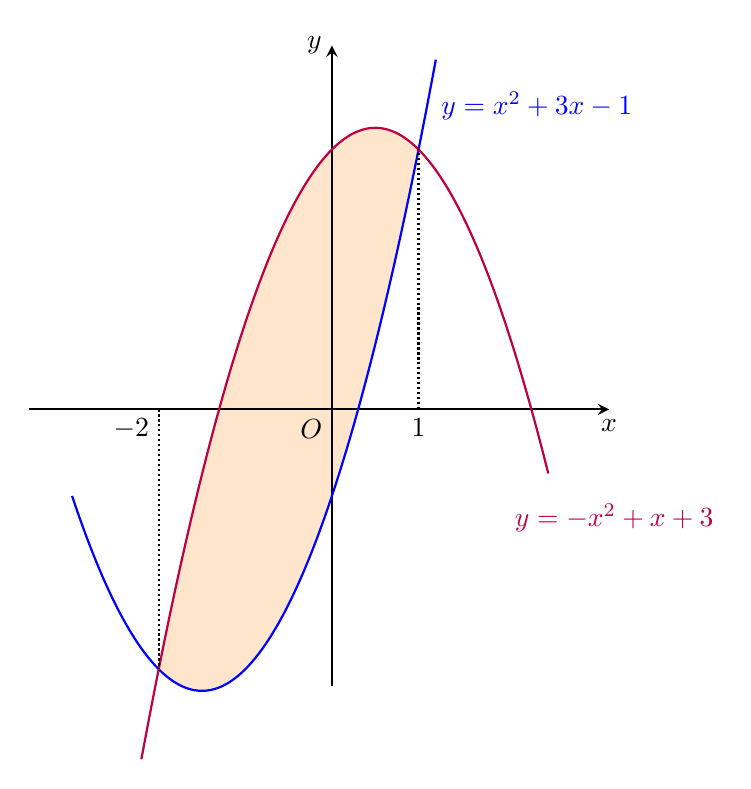
\begin{tikzpicture}[>=stealth,scale=1.1]
		\fill[orange!40,opacity=0.5]
		plot[domain=-2:1,samples=200] (\x,{-\x*\x+\x+3})
		--
		plot[domain=1:-2,samples=200] (\x,{\x*\x+3*\x-1})
		-- cycle;
		\draw[->,thick] (-3.5,0)--(3.2,0) node[below] {$x$};
		\draw[->,thick] (0,-3.2)--(0,4.2) node[left] {$y$};
		\draw[blue,thick,smooth,domain=-3:1.2,samples=200]
		plot(\x,{\x*\x+3*\x-1});
		\draw[purple,thick,smooth,domain=-2.2:2.5,samples=200]
		plot(\x,{-\x*\x+\x+3});
		\draw[densely dotted,thick] (-2,0)--(-2,{-(-2)*(-2)+(-2)+3});
		\draw[densely dotted,thick] (1,0)--(1,{1*1+3*1-1});
		\node[below left] at (-2,0) {$-2$};
		\node[below left] at (0,0) {$O$};
		\node[below] at (1,0) {$1$};
		\node[blue,right] at (1.15,3.5) {$y=x^2+3x-1$};
		\node[purple,right] at (2,-1.25) {$y=-x^2+x+3$};
	\end{tikzpicture}
	\end{center}
	\choice
	{\True $\displaystyle\int \limits_{-2}^1\left(4-2x-2x^2\right)\mathrm{\,d}x$}
	{$\displaystyle\int \limits_{-2}^1\left(-4x-2\right)\mathrm{\,d}x$}
	{$\displaystyle\int \limits_{-2}^1\left(2x^2+2x-4\right)\mathrm{\,d}x$}
	{$\displaystyle\int \limits_{-2}^1\left(4x+2\right)\mathrm{\,d}x$}
	\loigiai{
		Diện tích phần tô đậm là $S=\displaystyle\int \limits_{-2}^1\left[\left(-x^2+x+3\right)-\left(x^2+3x-1\right)\right]\mathrm{\,d}x=\displaystyle\int \limits_{-2}^1\left(4-2x-2x^2\right)\mathrm{\,d}x$.
	}
\end{ex}

\begin{ex}%[1D6H3-2]
	Tập xác định của hàm số $y=\left(x+3\right)^{\tfrac{1}{3}}$ là
	\choice
	{$\mathbb{R}\setminus\{-3\}$}
	{$\mathbb{R}$}
	{$\left[-3;+\infty\right)$}
	{\True $\left(-3;+\infty\right)$}
	\loigiai{
		Hàm số $y=\left(x+3\right)^{\tfrac{1}{3}}$ là hàm lũy thừa với số mũ không nguyên nên hàm số đã cho xác định khi và chỉ khi $x+3>0\Leftrightarrow x>-3$.
		Vậy tập xác định của hàm số $y=\left(x+3\right)^{\tfrac{1}{3}}$ là $\mathscr{D}=\left(-3;+\infty\right)$.
	}
\end{ex}

\begin{ex}%[2D1N1-2]
	Cho hàm số $y=f(x)$ có bảng biến thiên như sau
	\begin{center}
		
\begin{tikzpicture}
			\tkzTabInit[nocadre=false, lgt=1.2, espcl=2.5]
			{$x$ / 0.8, $y'$ / 0.8, $y$ / 2.5}
			{$-\infty$, $-1$, $0$, $1$, $+\infty$}
			\tkzTabLine{ , +, 0, -, d, -, 0, +, }
			\tkzTabVar{-/ $-\infty$, +/ , -D+/ $-\infty$ / $+\infty$, -/ , +/ $+\infty$}
		\end{tikzpicture}
	\end{center}
	Hàm số đã cho nghịch biến trên khoảng nào dưới đây?
	\choice
	{$(-\infty;-1)$}
	{\True $(-1;0)$}
	{$(0;+\infty)$}
	{$(-1;1)$}
	\loigiai{
		Dựa vào bảng biến thiên hàm số $y=f(x)$ nghịch biến trên các khoảng $(-1;0)$ và $(0;1)$.
	}
\end{ex}

\begin{ex}%[2H5N1-2]
	Trong không gian $Oxyz$, cho mặt phẳng $(P)\colon 3x-y+z+1=0$. Trong các vectơ sau, vectơ nào không phải là vectơ pháp tuyến của mặt phẳng $(P)$?
	\choice
	{$\overrightarrow{n}_2=\left(3;-1;1\right)$}
	{$\overrightarrow{n}_3=\left(-3;1;-1\right)$}
	{$\overrightarrow{n}_4=\left(6;-2;2\right)$}
	{\True $\overrightarrow{n}_1=\left(-3;-1;-1\right)$}
	\loigiai{
		Mặt phẳng $(P)$ có một vectơ pháp tuyến là $\overrightarrow{n}=(3;-1;1)$.\\
		Do đó vectơ pháp tuyến của $(P)$ là $k\overrightarrow{n}=(3k;-k;k)$ với $k\ne0$.
	}
\end{ex}

\begin{ex}%[1D6H4-2]
	Nghiệm của phương trình $3^{x-1}=1$ là
	\choice
	{$x=-1$}
	{$x=0$}
	{\True $x=1$}
	{$x=2$}
	\loigiai{
		Ta có $3^{x-1}=1\Leftrightarrow 3^{x-1}=3^0\Leftrightarrow x-1=0\Leftrightarrow x=1$.
	}
\end{ex}

\begin{ex} %[1D9H2-4]
	Cho $A$ và $B$ là hai biến cố thỏa mãn $P(A)=0{,}3;P(B)=0{,}6$ và $P(A\cup B)=0{,}7$. Tính xác suất của biến cố $AB$.
	\choice
	{$0{,}4$}
	{$0{,}3$}
	{\True $0{,}2$}
	{$0{,}65$}
	\loigiai{
		Ta có $\mathrm{P}(A\cup B)=\mathrm{P}(A)+\mathrm{P}(B)-\mathrm{P}(AB)$\\
		$\Leftrightarrow \mathrm{P}(AB)=\mathrm{P}(A)+\mathrm{P}(B)-\mathrm{P}(A\cup B)=0,3+0,6-0,7=0,2$.
	}
\end{ex}

\begin{ex} %[1D2H2-4]
	Cho cấp số cộng $(u_n)$ có số hạng đầu $u_1=-2$ và công sai $d=-7$. Giá trị $u_6$ bằng
	\choice
	{$33$}
	{$-33$}
	{$37$}
	{\True $-37$}
	\loigiai{
		Ta có $u_6=u_1+5d=-2+5\cdot (-7)=-37$.
	}
\end{ex}

\begin{ex} %[2D1N4-1]
	Đường thẳng nào dưới đây là đường tiệm cận đứng của đồ thị hàm số $y=\dfrac{5x-1}{x+2}$?
	\choice
	{Đường thẳng $x=5$}
	{Đường thẳng $x=2$}
	{\True Đường thẳng $x=-2$}
	{Đường thẳng $y=5$}
	\loigiai{
		Tập xác định $\mathscr{D}=\mathbb{R}\setminus\{-2\}$.\\
		Ta có $\lim \limits_{x\to {-2}^{-}}\dfrac{5x-1}{x+2}=+\infty$, $\lim \limits_{x\to {-2}^{+}}\dfrac{5x-1}{x+2}=-\infty$.\\
		Suy ra đường thẳng $x=-2$ là đường tiệm cận đứng của đồ thị hàm số $y=\dfrac{5x-1}{x+2}$.
	}
\end{ex}

\begin{ex} %[2D4N1-1]
	Cho các hàm số $f(x)$ và $g(x)$ liên tục trên tập xác định. Mệnh đề nào sau đây \textbf{sai}?
	\choice
	{$\displaystyle\int kf(x)\mathrm{\,d}x=k\displaystyle\int f(x)\mathrm{\,d}x\,(k\ne0)$}
	{$\displaystyle\int \left[f(x)+g(x)\right]\mathrm{\,d}x=\displaystyle\int f(x)\mathrm{\,d}x+\displaystyle\int g(x)\mathrm{\,d}x$}
	{\True $\displaystyle\int f(x)g(x)\mathrm{\,d}x=\displaystyle\int f(x)\mathrm{\,d}x\cdot \displaystyle\int g(x)\mathrm{\,d}x$}
	{$\displaystyle\int f'(x)\mathrm{\,d}x=f(x)+C{,}\,(C\in \mathbb{R})$}
	\loigiai{
		Ta có
		\begin{itemize}
			\item $\displaystyle\int kf(x)\mathrm{\,d}x=k\displaystyle\int f(x)\mathrm{\,d}x\,(k\ne0)$. Đúng.
			\item $\displaystyle\int \left[f(x)+g(x)\right]\mathrm{\,d}x=\displaystyle\int f(x)\mathrm{\,d}x+\displaystyle\int g(x)\mathrm{\,d}x$. Đúng.
			\item $\displaystyle\int f'(x)\mathrm{\,d}x=f(x)+C{,}\,(C\in \mathbb{R})$. Đúng.
		\end{itemize}
	}
\end{ex}

\cauds
\begin{ex} %[2H5H2-4] [2H5H2-7] [2H5N2-2]
	Trong không gian $Oxyz$, cho đường thẳng $\Delta \colon \heva{&x=3+t\\&y=4+2t\,{,\,}t\in \mathbb{R}\\&z=-3-t}$ và mặt phẳng $(P)$ có phương trình $2x+y+z-1=0$.
	\choiceTF
		{Giao điểm của $\Delta$ và $(P)$ là $M(3;4;-3)$}
		{\True Góc giữa $\Delta$ và $(P)$ là $30^\circ$}
		{$\sin (\Delta {,\,}(P))=\dfrac{\sqrt{3}}{2}$}
		{Một vectơ chỉ phương của $\Delta$ là $\overrightarrow{u}=(3;4;-3)$}
	\loigiai{
	\begin{itemchoice}
		\itemch Gọi $M=\Delta \cap (P)$. Vì $M\in \Delta$ nên $M(3+t;4+2t;-3-t)$.\\
		Mà $M\in (P)$ nên $2\cdot (3+t)+4+2t-3-t-1=0\Leftrightarrow 6+2t+t=0\Leftrightarrow t=-2$.\\
		Vậy $M(1;0;-1)$.
		\itemch  Đường thẳng $\Delta$ có vectơ chỉ phương $\overrightarrow{u}=(1;2;-1)$.\\
		Mặt phẳng $(P)$ có vectơ pháp tuyến $\overrightarrow{n}=(2;1;1)$.\\
		$\sin (\Delta {,\,}(P))=\dfrac{\left|\overrightarrow{u}\cdot \overrightarrow{n}\right|}{\left|\overrightarrow{u}\right|\cdot \left|\overrightarrow{n}\right|}=\dfrac{|1\cdot 2+2\cdot 1+(-1)\cdot 1|}{\sqrt{1^2+2^2+(-1)^2}\cdot \sqrt{2^2+1^2+1^2}}=\dfrac{1}{2}$.\\
		Suy ra $(\Delta {,\,}(P))=30^\circ$.
		\itemch Dựa vào câu b) ta có $\sin (\Delta {,\,}(P))=\dfrac{1}{2}$.
		\itemch Đường thẳng $\Delta$ có vectơ chỉ phương $\overrightarrow{u}=(1;2;-1)$.
	\end{itemchoice}
	}
	\end{ex}

\begin{ex} %[2D1V4-2]
		Cho hàm số $y=\dfrac{mx^2+\left(3m^2-2\right)x-2}{x+3m}$ $(1)$ với $m$ là số thực
		\choiceTF
		{\True Có $2$ giá trị $m$ để góc giữa hai tiệm cận của đồ thị hàm số $(1)$ bằng $45^{\circ}$}
		{\True Khi $m=1$ đồ thị hàm số có 2 điểm cực trị}
		{\True Khi $m=1$ đồ thị hàm số có đường tiệm cận xiên là $y=x-2$}
		{Khi $m=1$ giao điểm của đường tiệm cận xiên và tiệm cận đứng của đồ thị hàm số là $I\left(3;-5\right)$}
		\loigiai{
			\begin{itemchoice}
				\itemch 
				\begin{itemize}
					\item Trường hợp $1$: $m=0$\\
					Khi đó $y=\dfrac{-2x-2}{x}$. Do đó đồ thị hàm số có đường tiệm cận đứng là $x=0$, đường tiệm cận ngang là $y=-2$. Do đó góc tạo bởi giữa hai tiệm cận là $90^\circ$.\\
					Vậy $m=0$ không thoả mãn.
					\item Trường hợp $2$: $m\ne0$\\
					Ta có $y=\dfrac{mx^2+\left(3m^2-2\right)x-2}{x+3m}=mx-2+\dfrac{6m-2}{x+3m}$.\\
					Để đồ thị hàm số có hai đường tiệm cận thì $6m-2\ne0\Leftrightarrow m\ne\dfrac{1}{3}$.\\
					Khi đó tiệm cận đứng của đồ thị hàm số là đường thẳng $\Delta _1\colon x=-3m$ và tiệm cận xiên của đồ thị hàm số là đường thẳng $\Delta _2\colon y=mx-2$.\\
					$\Delta _1$ có vectơ pháp tuyến $n_1=(1;0)$,\\ $\Delta _2$ có vectơ pháp tuyến $n_2=(m;-1)$.
					\begin{eqnarray*}
\text{Theo đề, ta có  }&&(\Delta _1{,\,}\Delta _2)=45^\circ\\&\Rightarrow &\cos (\Delta _1{,\,}\Delta _2)=\cos 45^\circ\\&\Rightarrow &\dfrac{|\overrightarrow{n_1}\cdot \overrightarrow{n_2}|}{|\overrightarrow{n_1}|\cdot |\overrightarrow{n_2}}|=\dfrac{\sqrt{2}}{2}\\&\Rightarrow &\dfrac{|1\cdot m+0\cdot (-1)|}{\sqrt{1^2+0^2}\cdot \sqrt{m^2+(-1)^2}}=\dfrac{\sqrt{2}}{2}\\&\Rightarrow &2|m|=\sqrt{2}\cdot \sqrt{m^2+1}\\&\Rightarrow &4m^2=2(m^2+1)\\&\Rightarrow &m^2=1\\&\Rightarrow &m=\pm1.
\end{eqnarray*}
				\end{itemize}
				Vậy có $2$ giá trị $m$ để góc giữa hai tiệm cận của đồ thị hàm số $(1)$ bằng $45^{\circ}$.
				\itemch Khi $m=1$ thì $y=\dfrac{x^2+x-2}{x+3}$.\\
				$y'=\dfrac{x^2+6x+5}{(x+3)^2}$\\
				$y'=0\Leftrightarrow \dfrac{x^2+6x+5}{(x+3)^2}=0\Rightarrow x^2+6x+5=0\Rightarrow \hoac{&x=-5\\&x=-1.}$\\
				Vì phương trình $y'=0$ có hai nghiệm phân biệt nên hàm số có $2$ điểm cực trị.
				\itemch Dựa vào câu a), khi $m=1$ thì đồ thị hàm số có tiệm cận xiên là đường thẳng $y=x-2$.
				\itemch Dựa vào câu a), khi $m=1$ thì đồ thị hàm số có tiệm cận đứng là đường thẳng $x=-3$ và tiệm cận xiên là đường thẳng $y=x-2$.\\
				Do đó giao điểm của hai đường tiệm cận có toạ độ là $I(-3;-5)$.
			\end{itemchoice}
		}
	\end{ex}

\begin{ex} %[1H8V5-3]
		Cho lăng trụ đứng $ABC.A'B'C'$ có đáy là tam giác đều cạnh $a$, cạnh bên bằng $2a$. Gọi $M$, $N$ lần lượt là trung điểm của $AB'$ và $AC'$.
		\choiceTF
		{Khoảng cách giữa $BC$ và $(A'B'C')$ bằng $a$}
		{\True Khoảng cách giữa $BC$ và $(AB'C')$ bằng khoảng cách giữa $A'$ và $(AB'C')$}
		{\True Khoảng cách $MN$ và $(A'B'C')$ bằng $a$}
		{\True Khoảng cách giữa $(A'B'C')$ và $(ABC)$ bằng $2a$}
		\loigiai{
			\begin{center}
				\begin{tikzpicture}[scale=.8,declare function={a=5; b=0.45*a; h=0.9*a;}]
					\path (0:0) coordinate (A)
					(-43:b) coordinate (C)
					(a,0) coordinate (B)
					\foreach \x in {A,B,C}{(\x)++(90:h) coordinate (\x1)};
					\path ($(A)!0.5!(B1)$) coordinate (M);
					\path ($(A)!0.5!(C1)$) coordinate (N);
					\draw[dashed] (B1)--(A)--(B);
					\draw (C1)--(A1)--(B1)--cycle (A1)--(A)--(C)--(C1) (B1)--(B)--(C) (A)--(C1);
					\foreach \x/\goc/\t in {A/180/A,B/-90/B,C/-50/C,A1/100/A',B1/85/B',C1/80/C',M/120/M,N/160/N}
					\draw[fill=black] (\x) circle (1pt) node[shift={(\goc:9pt)},font=\scriptsize]{$\t$};
				\end{tikzpicture}
			\end{center}
			\begin{itemchoice}
				\itemch Vì $BC\parallel (A'B'C')$ nên $d(BC,\,(A'B'C'))=d(B{,}\,(A'B'C'))=B'B=2a$.
				\itemch Vì $BC\parallel (AB'C')$ nên $d(BC{,}\,(AB'C'))=d(C{,\,}(AB'C'))$.\\
				Mà $(AB'C')$ đi qua trung điểm của $A'C$ nên $d(C{,\,}(AB'C'))=d(A'{,\,}(AB'C'))$.
				\itemch Trong $(AB'C')$ có $MN$ là đường trung bình của tam giác $AB'C'$. Suy ra $MN\parallel B'C'$.\\
				Do đó $MN\parallel (A'B'C')$ nên\\ $d(MN{,\,}(A'B'C'))=d(M{,\,}(A'B'C'))=\dfrac{1}{2}d(A{,\,}(A'B'C'))=\dfrac{1}{2}AA'=a$.
				\itemch Vì $(A'B'C')\parallel (ABC)$ nên $d((A'B'C'),\,(ABC))=AA'=2a$.
			\end{itemchoice}
		}
	\end{ex}

\begin{ex} %[2D4V2-6]
		Một bác thợ xây bơm nước vào bể chứa nước. Gọi $h(t)$ là thể tích nước bơm được sau $t$ phút. Cho $h'(t)=6at^2+2bt$ và ban đầu bể không có nước. Sau 3 phút thì thể tích nước trong bể là $90$ m$^3$, sau $6$ phút thì thể tích nước trong bể là $504$ m$^3$.
		\choiceTF
		{\True $h(3)=\displaystyle\int \limits_0^3\left(6at^2+2bt\right)\mathrm{\,d}t=90$}
		{\True $h(t)=\displaystyle\int \left(6at^2+2bt\right)\mathrm{\,d}t$}
		{\True $a,b$ là nghiệm của hệ phương trình $\heva{&54a+9b=90\\&432a+36b=504.}$}
		{Sau $9$ phút thể tích nước trong bể là $V=1460$ m$^3$}
		\loigiai{
			Vì ban đầu bể không có nước nên ta có $h(0)=0$.\\
			Sau $3$ phút thì thể tích nước trong bể là $90$ m$^3$ nên $h(3)=90$. Ta có
			\begin{eqnarray*}
&&\displaystyle\int \limits_0^3h'(t)\mathrm{\,d}t=90\\&\Leftrightarrow &\displaystyle\int \limits_0^3(6at^2+2bt)\mathrm{\,d}t=90\\&\Leftrightarrow &(2at^3+bt^2)\biggl|_0^3=90\\&\Leftrightarrow &54a+9b=90.\quad(1)
\end{eqnarray*}
			Sau $6$ phút thì thể tích nước trong bể là $90$ m$^3$ nên $h(6)=504$. Ta có
			\begin{eqnarray*}
&&\displaystyle\int \limits_0^6h'(t)\mathrm{\,d}t=504\\&\Leftrightarrow &\displaystyle\int \limits_0^6(6at^2+2bt)\mathrm{\,d}t=504\\&\Leftrightarrow &(2at^3+bt^2)\biggl|_0^6=504\\&\Leftrightarrow &432a+36b=504.\quad(2)
\end{eqnarray*}
			Từ $(1)$ và $(2)$, ta có hệ phương trình $\heva{&54a+9b=90\\&432a+36b=504}\Leftrightarrow \heva{&a=\dfrac{2}{3}\\&b=6.}$
			Vậy $h'(t)=4t^2+12t$. 
			\begin{itemchoice}
				\itemch Vì $\displaystyle\int \limits_0^3\left(6at^2+2bt\right)\mathrm{\,d}t=h(t)\biggl|_0^3=h(3)-h(0)=h(3)\Rightarrow h(3)=90$.
				\itemch Ta có $h(t)=\displaystyle\int (6at^2+2bt)\mathrm{\,d}t$.
				\itemch Dựa vào lời giải phía trên.
				\itemch Sau $9$ phút thì thể tích nước trong bể là 
				\begin{eqnarray*}
V&=&h(9)=\displaystyle\int \limits_0^9h'(t)\mathrm{\,d}t\\&=&\displaystyle\int \limits_0^9(4t^2+12t)\mathrm{\,d}t\\&=&1458\,(\text{m}^3).
\end{eqnarray*}
			\end{itemchoice}
		}
	\end{ex}

\caukq
\begin{ex} %[1H8V6-2]
	Cho hình lập phương $ABCD.A'B'C'D'$ có cạnh bằng $a$. Tính số đo của góc nhị diện $\left[B,A'C,D\right]$.
	\shortans{120}
	\loigiai{
		\begin{center}
				\begin{tikzpicture}[scale=1,declare function={r=2.8;},font=\scriptsize]
				\path (0:0) coordinate (A)
				(0:r+0.5) coordinate (B)
				++(37:{0.65*r}) coordinate (C)
				++(180:r+0.5) coordinate (D)
				\foreach \x in {A,B,C,D}{(\x)++(90:r) coordinate (\x_1)};
				\path ($(A_1)!0.8!(C)$) coordinate (H);
				\draw[dashed] (D_1)--(D)--(A) (A_1)--(D)--(C)--cycle (B)--(D)--(H)--cycle;
				\draw (A)--(B)--(C) (A)--(A_1) (B)--(B_1) (C)--(C_1)(A_1)--(B_1)--(C_1)--(D_1)--cycle;
				\foreach \x/\goc/\t in {A/255/A, B/-75/B, C/10/C, D/170/D, A_1/135/A', B_1/90/B',
					C_1/45/C', D_1/90/D', H/70/H}{
					\draw[fill=black] (\x) circle (1pt) node[shift={(\goc:9pt)}]{$\t$};
					\foreach \x/\y/\z in {B/H/C,D/H/A_1}{
						\path (\y) pic[draw=black,angle radius=5pt]{right angle = \x--\y--\z};
					};
				}
			\end{tikzpicture}
		\end{center}
		Ta có $BD\perp \left(AA'C'C\right)\Rightarrow BD\perp A'C$.\\
		Trong mặt phẳng $\left(A'DC\right)$ kẻ $DH\perp A'C$. Suy ra $A'C\perp (BDH)\Rightarrow A'C\perp BH$.\\
		Ta có $\heva{&(A'BC)\cap (A'DC)=A'C\\&BH\perp A'C{,\,}BH\subset (A'BC)\\&DH\perp (A'DC){,\,}DH\subset (A'DC)}$. \\
		Suy ra góc phẳng nhị diện $\left[B,A'C,D\right]$ là góc giữa $(BH{,\,}DH)=\widehat{BHD}$.\\
		Xét tam giác $A'DC$ vuông tại $D$ có $A'D=a\sqrt{2}$, $DC=a$, $A'C=a\sqrt{3}$
		\begin{eqnarray*}
&&DH.A'C=A'D.DC\\&\Leftrightarrow &DH=\dfrac{A'D\cdot DC}{A'C}\\&\Leftrightarrow &DH=\dfrac{a\sqrt{2}\cdot a}{a\sqrt{3}}\\&\Leftrightarrow &DH=\dfrac{a\sqrt{6}}{3}.
\end{eqnarray*}
		Vì $\Delta A'BC=\Delta A'DC$ nên $BH=DH$.\\
		Xét tam giác $BDH$ có 
		\begin{eqnarray*}
&BD^2&=BH^2+DH^2-2BH.DH\cdot \cos \widehat{BHD}\\&\Leftrightarrow &2a^2=\dfrac{2a^2}{3}+\dfrac{2a^2}{3}-2\cdot \dfrac{2a^2}{3}\cos \widehat{BHD}\\&\Leftrightarrow &\cos \widehat{BHD}=-\dfrac{1}{2}\\&\Leftrightarrow &\widehat{BHD}=120^{\circ}.
\end{eqnarray*}
		Vậy $[B,A'C,D]=120^\circ$.
	}
\end{ex}

\begin{ex} %[2D6V2-4]
	Một xét nghiệm Covid--$19$ cho kết quả dương tính với $90\%$ các trường hợp thực sự nhiễm virus và cho kết quả âm tính với $80\%$ các trường hợp thực sự không nhiễm virus. Biết rằng tỉ lệ người nhiễm Covid--$19$ trong một cộng đồng nào đó là $1\%$. Một người trong cộng đồng đó cho kết quả xét nghiệm dương tính. Xác suất để người đó thực sự bị nhiễm virus có dạng $\dfrac{a}{b}$. Giá trị của $a+b$ bằng bao nhiêu?
	\shortans{24}
	\loigiai{
		Gọi $A$ là biến cố \lq\lq Người đó bị nhiễm Virus\rq\rq.\\
		$B$ là biến cố \lq\lq Người đó cho kết quả dương tính\rq\rq.\\
		Ta có $\mathrm{P}\left(B|A\right)=0{,}9$; $\mathrm{P}\left(B|\overline{A}\right)=0{,}2$; $\mathrm{P}\left(A\right)=0{,}01\Rightarrow \mathrm{P}\left(\overline{A}\right)=0{,}99$.\\
		Do đó xác suất để người đó cho kết quả dương tính là
		$$\mathrm{P}\left(B\right)=\mathrm{P}\left(A\right)\cdot \mathrm{P}\left(B|A\right)+\mathrm{P}\left(\overline{A}\right)\cdot \mathrm{P}\left(B|\overline{A}\right)=0{,}01\cdot 0{,}9+0{,}99\cdot 0{,}2=0{,}207.$$
		Xác suất để người nhiễm virus cho kết quả dương tính là
		$$\mathrm{P}\left(A|B\right)=\dfrac{\mathrm{P}\left(A\right)\cdot \mathrm{P}\left(B|A\right)}{\mathrm{P}\left(B\right)}=\dfrac{0{,}01\cdot 0{,}9}{0{,}207}=\dfrac{1}{23}.$$
		Vậy $a=1$, $b=23\Rightarrow a+b=24$.
	}
\end{ex}

\begin{ex} %[2D1V4-4]
	Giả sử dân số của một huyện sau $t$ năm kể từ năm 2024 được mô tả bởi hàm số $f(t)=\dfrac{20t+5}{t+2}$, $t\ge 0$. Dân số của huyện đó luôn tăng nhưng không vượt quá bao nhiêu nghìn người?
	\shortans{20}
	\loigiai{
		Ta có $\lim \limits_{t\to +\infty}f(t)=\lim \limits_{t\to +\infty}\dfrac{20t+5}{t+2}=20$.\\
		Vậy dân số của huyện đó không vượt quá $20$ nghìn người.
	}
\end{ex}

\begin{ex} %[2D4V3-1]
	Trong mặt phẳng tọa độ $Oxy$, cho hình thang $OABC$ có $A(0;4)$, $B(5;2)$, $C(5;0)$. Thể tích khối tròn xoay tạo thành khi quay hình thang $OABC$ quanh trục $Ox$ bằng bao nhiêu? Làm tròn đến hàng đơn vị.
	\begin{center}
		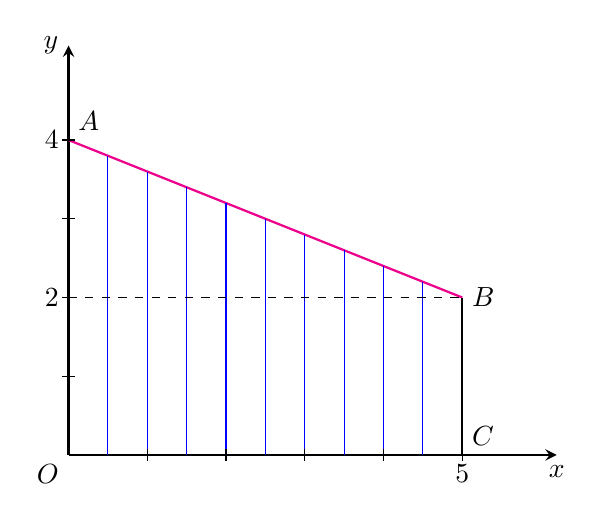
\begin{tikzpicture}[scale=1,>=stealth]
			\draw[->,thick] (0,0)--(6.2,0) node[below] {$x$};
			\draw[->,thick] (0,0)--(0,5.2) node[left] {$y$};
			\coordinate (A) at (0,4);
			\coordinate (B) at (5,2);
			\coordinate (C) at (5,0);
			\coordinate (O) at (0,0);
			\draw[thick,magenta] (A)--(B);
			\draw[thick] (B)--(C);
			\draw[thick] (O)--(C);
			\foreach \x in {0.5,1,1.5,2,2.5,3,3.5,4,4.5} {
				\pgfmathsetmacro{\yy}{4-0.4*\x}
				\draw[blue] (\x,0)--(\x,\yy);
			}
			\foreach \x in {1,2,3,4,5}
			\draw (\x,0.08)--(\x,-0.08);
			\foreach \y in {1,2,3,4}
			\draw (0.08,\y)--(-0.08,\y);
			\draw[dashed] (0,2)--(5,2);
			\node[above right] at (A) {$A$};
			\node[left] at (A) {$4$};
			\node[right] at (B) {$B$};
			\node[above right] at (C) {$C$};
			\node[below left] at (O) {$O$};
			\node[left] at (0,2) {$2$};
			\node[below] at (5,0) {$5$};
		\end{tikzpicture}
	\end{center}
	\shortans{147}
	\loigiai{
		Phương trình đường thẳng $AB$ có dạng $y=ax+b$.\\
		Đường thẳng $AB$ đi qua $A\left(0;4\right),B\left(5;2\right)$ nên ta có hệ phương trình $\heva{&b=4\\&5a+b=2}\Leftrightarrow \heva{&a=-\dfrac{2}{5}\\&b=4.}$\\
		Suy ra phương trình đường thẳng $AB$ là $y=-\dfrac{2}{5}x+4$.\\
		Thể tích của khối tròn xoay tạo thành khi quay hình thang $OABC$ quanh trục $Ox$ là $$V=\pi\displaystyle\int \limits_0^5\left(-\dfrac{2}{5}x+4\right)^2\mathrm{\,d}x=\dfrac{140}{3}\pi\approx147\,\text{(đvtt).}$$
	}
\end{ex}

\begin{ex} %[2H5V2-7]
	Khi gắn hệ tọa độ $Oxyz$ vào một căn nhà sao cho nền nhà thuộc mặt phẳng $\left(Oxy\right)$, người ta coi mỗi mái nhà là một phần của mặt phẳng và thấy ba vị trí $A$, $B$, $C$ ở mái nhà bên phải lần lượt có tọa độ $\left(1;0;3\right)$, $\left(5;0;1\right)$ và $\left(5;9;1\right)$. Góc giữa mái nhà bên phải và nền nhà bằng bao nhiêu độ?
	\shortans{27}
	\loigiai{
		Mặt phẳng $(ABC)$ có cặp vectơ chỉ phương là $\overrightarrow{AB}=(4;0;-2)$ và $\overrightarrow{AC}=(4;9;-2)$.\\
		Suy ra mặt phẳng $(ABC)$ có vectơ pháp tuyến là $\overrightarrow{n}=\left[\overrightarrow{AB},\overrightarrow{AC}\right]=(18;0;36)$.\\
		Do đó vectơ $\overrightarrow{n}_1=\dfrac{1}{18}\overrightarrow{n}=(1;0;2)$ cũng là vectơ pháp tuyến của $(ABC)$ và $(Oxy)$ có vectơ pháp tuyến là $\overrightarrow{n}_2=(0;0;1)$.\\
		Ta có $\cos ((ABC){,\,}(Oxy))=\dfrac{\left|\overrightarrow{n}_1\cdot \overrightarrow{n}_2\right|}{\left|\overrightarrow{n}_1\right|\cdot \left|\overrightarrow{n}_2\right|}=\dfrac{|1\cdot 0+0\cdot 0+2\cdot 1|}{\sqrt{1^2+0^2+2^2}\cdot \sqrt{0^2+0^2+1^2}}=\dfrac{2\sqrt{5}}{5}$.\\
		Vậy $((ABC){,\,}(Oxy))\approx27^{\circ}$.
	}
\end{ex}

\begin{ex} %[2H2V1-4]
	Ở một sân bay, vị trí của máy bay được xác định bởi điểm $M$ trong không gian $Oxyz$ như hình vẽ. Gọi $H$ là hình chiếu vuông góc của $M$ xuống mặt phẳng $(Oxy)$. Biết $OM=79$; $\left(\overrightarrow{i}{,\,}\overrightarrow{OH}\right)=68^{\circ}$; $\left(\overrightarrow{OH}{,\,}\overrightarrow{OM}\right)=50^{\circ}$. Gọi toạ độ điểm $M(a;b;c)$. Giá trị của $a+b+c$ là bao nhiêu, kết quả làm tròn đến hàng đơn vị?
	\begin{center}
		\begin{tikzpicture}[x={(-0.6cm,-0.4cm)}, y={(1cm,0cm)}, z={(0cm,1cm)}, scale=1,>=stealth]
			\coordinate (O) at (0,0,0);
			\coordinate (A) at (3,0,0);
			\coordinate (B) at (0,4,0);
			\coordinate (C) at (0,0,3);
			\coordinate (H) at (3,4,0);
			\coordinate (M) at (3,4,3);
			\draw[->, thick] (0,0,0) -- (5.5,0,0) node[below] {$x$};
			\draw[->, thick] (0,0,0) -- (0,5.5,0) node[below] {$y$};
			\draw[->, thick] (0,0,0) -- (0,0,4.5) node[left] {$z$};
			\draw[dashed, thick] (A) -- (H) -- (B) (O) -- (H) (H) -- (M) (C) -- (M);
			\foreach \x/\y/\z in {H/A/O,H/B/O,O/C/M}{
				\path (\y) pic[draw,angle radius=5pt]{right angle = \x--\y--\z};
			}
			\draw[->, thick] (O) -- (1.5,0,0) node[midway, above left] {$\overrightarrow{i}$};
			\draw[->, thick] (O) -- (0,1.5,0) node[midway, above right] {$\overrightarrow{j}$};
			\draw[->, thick] (O) -- (0,0,1.5) node[midway, left] {$\overrightarrow{k}$};
			\foreach \t/\g in {O/-80, A/90, B/90, C/150, H/-90, M/90}{
				\draw[fill=black] (\t) circle (1pt) node[shift={(\g:9pt)},font=\scriptsize]{$\t$};
			}
			\draw[->, thick, blue!70!black] (O) -- (M);
		\end{tikzpicture}
	\end{center}
	\shortans{127}
	\loigiai{
		Ta có $OC=MH=OM\sin \widehat{HOM}=79\sin 50^{\circ}$. \\ 
		$OH=OM\cos \widehat{HOM}=79\cos 50^{\circ}$. \\ 
		$OA=OH\cos \widehat{AOH}=79\cos 50^{\circ}.\cos 68^{\circ}$. \\ 
		$OB=AH=OH\sin \widehat{AOH}=79\cos 50^{\circ}\cdot \sin 68^{\circ}$.\\
		Suy ra $\heva{&a=79\cos 50^{\circ}\cdot \cos 68^{\circ}\\&b=79\cos 50^\circ\cdot \sin 68^{\circ}\\&c=79\sin 50^{\circ}}$. Vậy $a+b+c\approx127$.
	}
\end{ex}

\Closesolutionfile{ans}
\indapan{4}{ans/De-TB-Yeu-So-17}
